\documentclass[a4paper]{article}

\usepackage[utf8]{inputenc}
\usepackage[T1]{fontenc}
\usepackage{amsmath}
\usepackage{graphicx}
\usepackage{fancyhdr}
\usepackage{tabularx}
\usepackage{listingsutf8}
\usepackage{hyperref}
\usepackage{etoolbox}% http://ctan.org/pkg/etoolbox
\usepackage{needspace}% http://ctan.org/pkg/needspace

% Für Theoreme (Beispiele, Definitionen, Sätze etc.)
\usepackage{amsthm}

\usepackage[colorinlistoftodos,prependcaption,textsize=tiny]{todonotes}

%\Bearbeitet Format, sodass statt der Einrückung bei Paragraphen durch Zeilenabstand ersetzt wird
\usepackage{parskip}
\setlength\parindent{0pt}

%\Setzt Dokumentinformationen
\title{Master-Thesis: Incremental Analysis of Software Product Lines}
\author{Moritz Fl\"oter}
\date{June 2018}



\begin{document}
\bibliographystyle{unsrt}

\newtheoremstyle{mystyle}% name
  {3pt}%Space above
  {3pt}%Space below
  {\normalfont}%Body font
  {0pt}%Indent amount
  {\bfseries}% Theorem head font
  {}%Punctuation after theorem head
  {\newline}%Space after theorem head 2
  {}%Theorem head spec (can be left empty, meaning 'normal')

\theoremstyle{mystyle}


\newtheorem{req}{REQ}
\newtheorem{subreq}{REQ}[req]
\newtheorem{subsubreq}{REQ}[subreq]
\AtBeginEnvironment{req}{\Needspace{5\baselineskip}}
\setcounter{req}{0}

\newcommand*{\reqtable}[4]{
\begin{tabular}{ | p{0.15\textwidth} | p{0.79\textwidth} | }
	\hline
	\textit{Priority} & \begin{minipage}[l]{0.79\textwidth}
	\vspace{0.25em}
		#1
	\vspace{0.25em}
	\end{minipage} \\ \hline
	\textit{Source} & \begin{minipage}[l]{0.79\textwidth}
	\vspace{0.25em}
		#2
	\vspace{0.25em}
	\end{minipage}\\ \hline
	\textit{Description} & \begin{minipage}[l]{0.79\textwidth}
	\vspace{0.25em}
		#3
	\vspace{0.25em}
	\end{minipage} \\ \hline
	\textit{Explanation} & \begin{minipage}[l]{0.79\textwidth} 
	\vspace{0.25em}
		#4
	\vspace{0.25em}
	\end{minipage} \\
	\hline
\end{tabular}
}



%\Deckblatt
\maketitle
\newblock

\begin{center}
floeter@uni-hildesheim.de \par
Matrikel-Nr: 236278 \par
Supervisor: \par
Prof. Dr. Klaus Schmid \par
Christian K\"oher
\end{center}

\newpage
\lhead{{}}
\rhead{\leftmark}
\pagestyle{fancy}

\listoftodos[Notes]
\clearpage

%\Inhaltsverzeichnis
\tableofcontents
\newpage
\bibliographystyle{unsrt}

%\Deckblatt
\maketitle
\newpage

\setcounter{page}{1}
\lhead{{}}
\rhead{\leftmark}
\pagestyle{fancy}



\section{Introduction}

\todo{Nicht vergessen: Aufbau der Arbeit erneut beschreiben}

\section{Background}
\subsection{Software Product Lines}

\subsection{Software Product Line Analyses}

\subsection{KernelHaven - an Analysis Infrastructure}\label{kernelhaven}

\todo{describe extension possiblities - plugins, preparation task etc.}

\todo{describe phases in non-incremental infrastructure}

\subsection{Objective for this Work}


\clearpage
\section{Requirements for the Software System}

\begin{req}[Working Base of Incremental Analysis]
	\reqtable
	{Must}  {Interview}
	{The incremental analysis must work based on the current state of a repository and a proposed change}
	{The working base of each incremental analysis is the previous state before a commit/code change. The increment is represented by the change introduced.}
	
	\begin{subreq}[Input Format for Incremental Analysis] \label{req:git-diff}
		\reqtable
		{Must}  {Interview}
		{The input must be a git-diff. Furthermore a filebase upon which the diff can be applied is required.}
		{The main input for the analysis is a git-diff. This diff represents a changeset that is to be analysed.}
	\end{subreq}
\end{req}

\begin{req}[Covered Analysis-Types]
	\reqtable
	{Must}  {Initial Description, Interview}
	{The incremental analysis must support block-based analyses.}
	{}
	
	\begin{subreq}[Input Format for Incremental Analysis] \label{req:git-diff}
		\reqtable
		{Must}  {Interview}
		{The input must be a git-diff}
		{The main input for the analysis is a git-diff. This diff represents a changeset that is to be analysed.}
	\end{subreq}
\end{req}


\begin{req}[Filtering of Source Files] \label{req:early-filtering}
\reqtable
	{Must}  {Interview}
	{The set of source files upon which the analysis operates should be reduced before being passed to the extractors.}
	{Because extraction is costly, the filtering of artifacts must happen on a file basis before the extractors are called.}
\end{req}

\clearpage
\begin{req}[Configuration of Filters for Input-Files] \label{req:optimization}
\reqtable
	{Must}  {Initial Description}
	{
	The implemented infrastructure must provide means to configure different filters for the files that are to be analyzed.
    }
	{Depending on the extractor in use and the way it processes input files, different options cover different use cases. Furthermore different filters may affect the overall performance of the software system.}

\begin{subreq}[Implementation of Filters for Input-Files]
    \reqtable
	{Must}  {Interview, initial description}
	{
	The filters listed below must be implemented (see REQ \ref{req:optimization}):
	\begin{itemize}
		\item \texttt{off} \\
		no filtering 
	    \item \texttt{change only} \\
	    only work with files that were modified
	    \item \texttt{variability-change only} \\
	     only work with files where the variability information was changed
	\end{itemize}
    }
	{In order to evaluate different filter methods and their effect on performance, different categories of filtering are required. \texttt{off} represents the state where no filtering is done, while \texttt{change only} performs superficial filtering without regarding variability information directly. Finally \texttt{variability-change only} is the most sophisticated filtering option of the three as it requires an analysis of the filecontent of each artifact itself.}
\end{subreq}

\begin{subreq}[Implementation of Effect-Filters for Input-Files]
    \reqtable
	{May}  {Interview, initial description}
	{
	The filters listed below may be implemented:
	\begin{itemize}
		\item \texttt{change-effect} \\
		work with files that were modified and files that were indirectly affected by the change (eg. through includes)
	    \item \texttt{variability-effect}  \\
	    work with files where the variability information was changed and files that were indirectly affected by the variability change
	\end{itemize}
    }
	{When a file is modified, it may affect other files as well that were not changed directly. Depending on the extractors and analyses used it may be necessary to analyze those files as well.}
\end{subreq}

\end{req}

\begin{req}[Rollback must be possible] \label{req:rollback}
\reqtable
	{Must}  {Interview}
	{It must be possible to revert back to the previous state after execution of an incremental analysis.}
	{An Analysis may change the source-files used as input for the extractors along with other changes. Those changes reflect the changes introduced by the new increment that was used as input. If that increment however contains defects identified by the analysis the user might choose to revert the changes and propose an alternative change. This alternative change can only be analyzed if KernelHaven reverts to the original state before the initial change.}

\end{req}

\begin{req}[Incremental Dead Code Analysis] 
\reqtable
	{Must}  {Initial description}
	{An incremental dead code analysis must be integrated in the software system}
	{The dead code analyis serves as a practical example for block based analyses. It is used to demonstrate and evaluate the effectiveness of the incremental approach.}
	
	

	
	\begin{subreq}[Incremental Dead Code Analysis Result Format] \label{req:format}
    \reqtable
    {Must}  {Interview}
	{The result should be given in the same csv-format as implemented in the existing UnDeadAnalyzer\footnote{\url{https://github.com/KernelHaven/UnDeadAnalyzer}} plugin for Kernelhaven. If no new analysis is required, a message should be printed to the log and no new result-file must be generated as output.}
	{Maintaining the same format as the non-incremental dead code analysis allows for comparability between incremental and non-incremental analyses. In contrast to non incremental analyses there might be situations where no new analysis is required. If that is the case, a message must be written to the log. However no new result-file has to be generated. \\
	\emph{Note: eventhough the csv-format remains unchangend, the contents of incremental and non-incremental result-files might differ (see REQ \ref{req:coverage})}}
	\end{subreq}
	
	\begin{subreq}[Incremental Dead Code Analysis Result Coverage] \label{req:coverage}
    \reqtable
    {Must}  {Interview, feedback from presentation of initial concept}
	{The analyis result should only contain elements that are results of the latest analysis increment}
	{As the analysis should provide feedback for the developer on his work, parts of the software system which could not have been affected by the changes he introduced do not need to be represented in the result. Therefore merging the result of the increment with previous results is not desired.}
	\end{subreq}
\end{req}

\clearpage
\begin{req}[Target Artifacts] 
\reqtable
    {Must}  {Initial Description}
	{The software system must support the processing of *.c, *.h, makefile, Kbuild and Kconfig files}
	{The filetypes listed above represent the CodeModel, BuildModel and VariabilityModel of the Linux kernel. As the Linux kernel is used for the evaluation of the implemented incremental analysis approach, those filetypes need to be considered.}
\end{req}





\begin{req}[Run existing KernelHaven-Analyses incrementally] 
\reqtable
    {May}  {Interview \\ \emph{Note: This requirement emerged after the implementation choice to use the KernelHaven infrastructure}}
	{It should be possible to run existing analyses incrementally without reimplementation.}
	{Existing analysis plugins for KernelHaven have been written as non-incremental analyses. The adaptation of existing analyses removes the need to reimplement existing analyses. Furthermore the adaptation of existing plugins allows for performance evaluation of incremental analyses against non-incremental analyses.}
\end{req}

\newpage

\section{Implementation of Incremental Analyses}

This section describes the implemented infrastructure for incremental analyses and provides reasoning for the decisions made when engineering the infrastructure. The term 'incremental analyses' will henceforth be used as shorthand for  'block based incremental analyses' as other types of analyses are not targeteted by the infrastructure.

The infrastructure itself is based on KernelHaven\cite{KernelHaven} as KernelHaven together with its plugins provides a working implementation for various software product line analyses. Through KernelHaven's plugin interfaces, it is also possible to implement the infrastructure for incremental analyses as a plugin itself.

By extending an existing infrastructure like KernelHaven, we can benefit from an existing codebase as well as future developments within the KernelHaven project. Furthermore future users of the incremental infrastructure can adjust existing non-incremental analyses written for KernelHaven to run as incremental analyses.

\subsection{Overview: Four Phases of an Incremental Analysis}


A simple non-incremental analysis in KernelHaven can be broken down to phases: the extraction phase and the analysis phase. In the extraction phase, KernelHaven extracts models from the codebase. In the analysis-phase the resulting models are used to compute the analysis results. A configuration file defines where the codebase is located and provides settings for the extractors and analysis. From the standpoint of an analysis-developer, the configuration file directly defines the configuration for extractors and analysis. The implementation within KernelHaven is more complex as the configuration is read and transferred into a Configuration-object that is then made available to extractors and analyses. For simplification purposes this process is not represented in detail within the illustration. 

\begin{figure}[h] 
  \centering
  \begin{minipage}[b]{0.7\textwidth} 
    \caption[Non-Incremental Analysis: Two Phases]{Non-Incremental Analysis: Two Phases}\label{2-phases}
    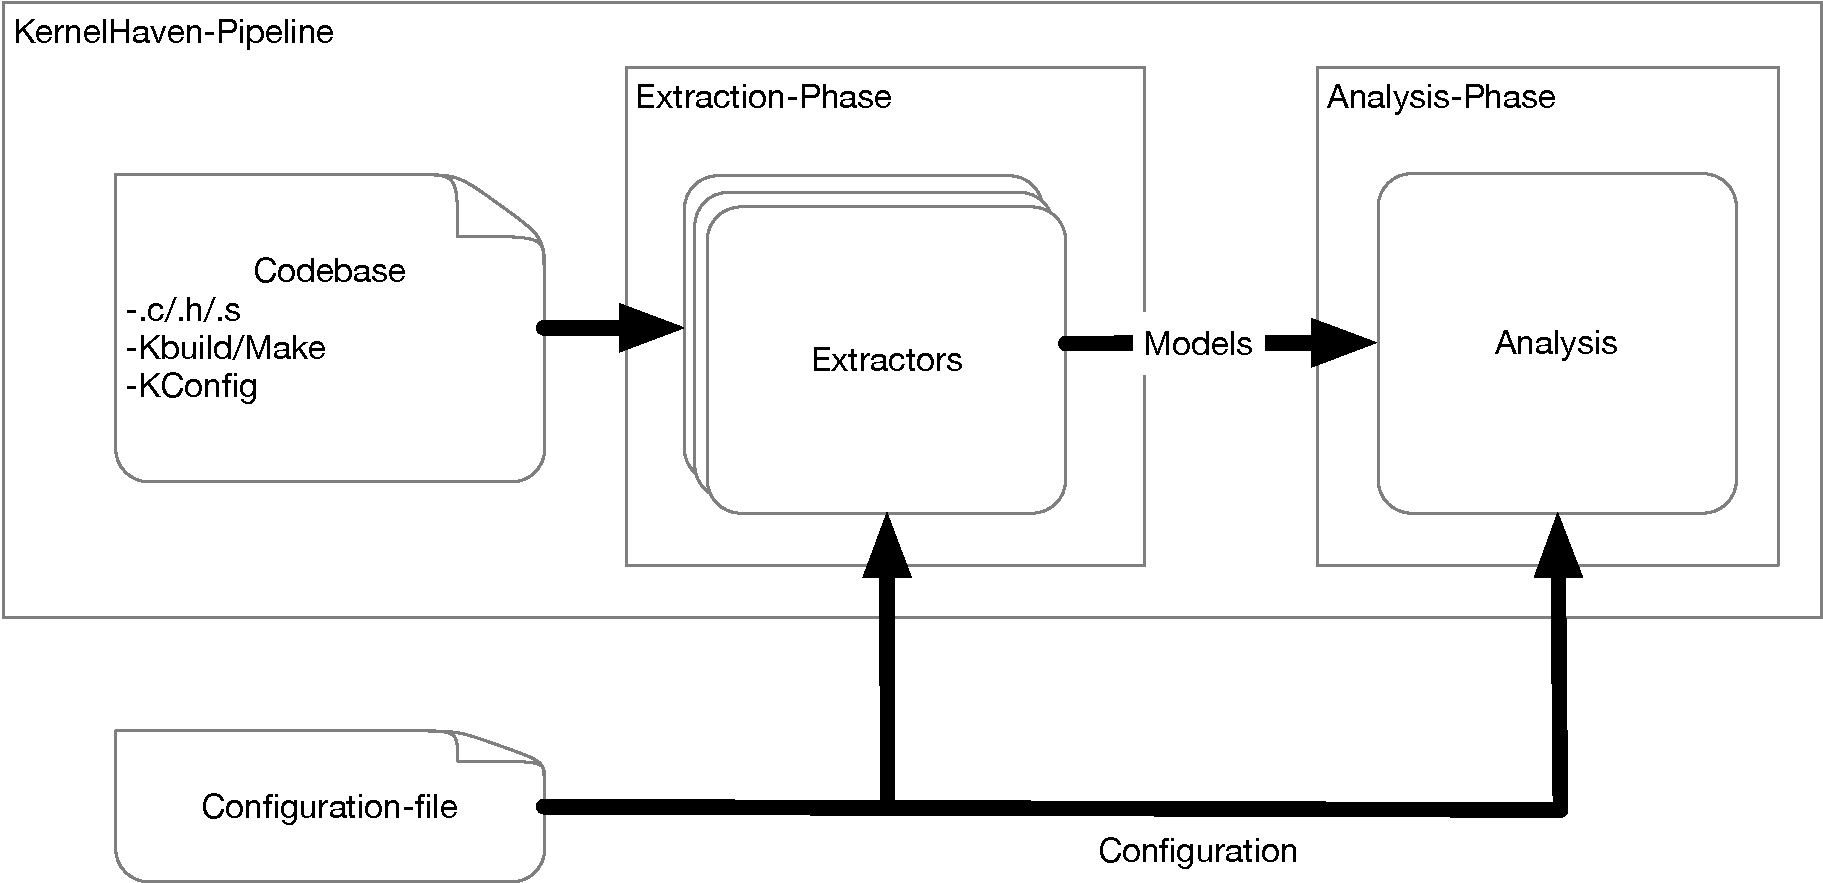
\includegraphics[width=1\textwidth]{img/KernelHaven.pdf}
  \end{minipage}
\end{figure}

While the Analysis- and Extraction-Phase are also present for analyses implemented with the incremental infrastructure, there are additional mandatory tasks which get executed in two more phases - the Preparation-Phase and the Post-Extraction-Phase. The resulting four phases are visualized in \autoref{4-phases}.

The Preparation-Phase is the first phase in an incremental analysis. Its purpose is to update the codebase and reduce the number of files that the extraction has to run on (see REQ \ref{req:early-filtering}. This saves computational effort when running the extractors as some parts of the codebase  may not need to be processed again. Instead the result of previous extractions may be reused. KernelHaven allows the configuration-object to define which files extractors run on. Therefore the configuration is not simply read from the configuration-file and passed on without modification but instead gets modified to only define a subset of the original files. This modification happens in the Preparation-Phase before the Extraction-Phase starts.

 But even before any filtering on the artifacts in the codebase happens, the incremental infrastructure ensures that the codebase represents the increment that is to be analyzed. This is possible to achieve by using a git-diff file describing changes to the codebase (see REQ \ref{req:git-diff}). In order to allow for reuse of existing extractors, the changes need to be applied to the codebase on the filesystem as the extractor-plugins for KernelHaven work based on access to the filesystem and can not work with data streams.

Because of the filtering performed in the Preparation-Phase, the analysis may not simply run on the result of the extractors directly as those would only generate a subset of the models. Therefore the result is merged with the results of previous extractions. After merging, it makes the resulting code-, build- and variabilitymodel available to the analysis through the \texttt{HybridCache}.

While merging the extractors outputs, it is important that no prior extraction results get overwritten. This is because REQ \ref{req:rollback} requires that the state before the execution of an incremental analysis can be restored. Therefore the Post-Extraction-Phase uses a modified implementation of the cache-system, that the main infrastructure of KernelHaven uses. This \texttt{HybridCache} allows storage and access to two versions of the code-, build- and variabilitymodel. It guarantees that the previous code-, build- and variabilitymodel can be restored.

While a rollback to previous extraction-results is the main reason for introducing the \texttt{HybridCache}, a side benefit is that analyses now may use both the current and the previous state of the codebase. This could be relevant for future implementations of incremental analyses that draw benefits from comparing the old and the new model. \todo{eventually discuss this in more detail? or reference to a later chapter}.

\begin{figure}[h] 
  \centering
  \begin{minipage}[b]{1\textwidth} 
    \caption[Incremental Analysis: Four Phases]{Incremental Analysis: Four Phases}\label{4-phases}
    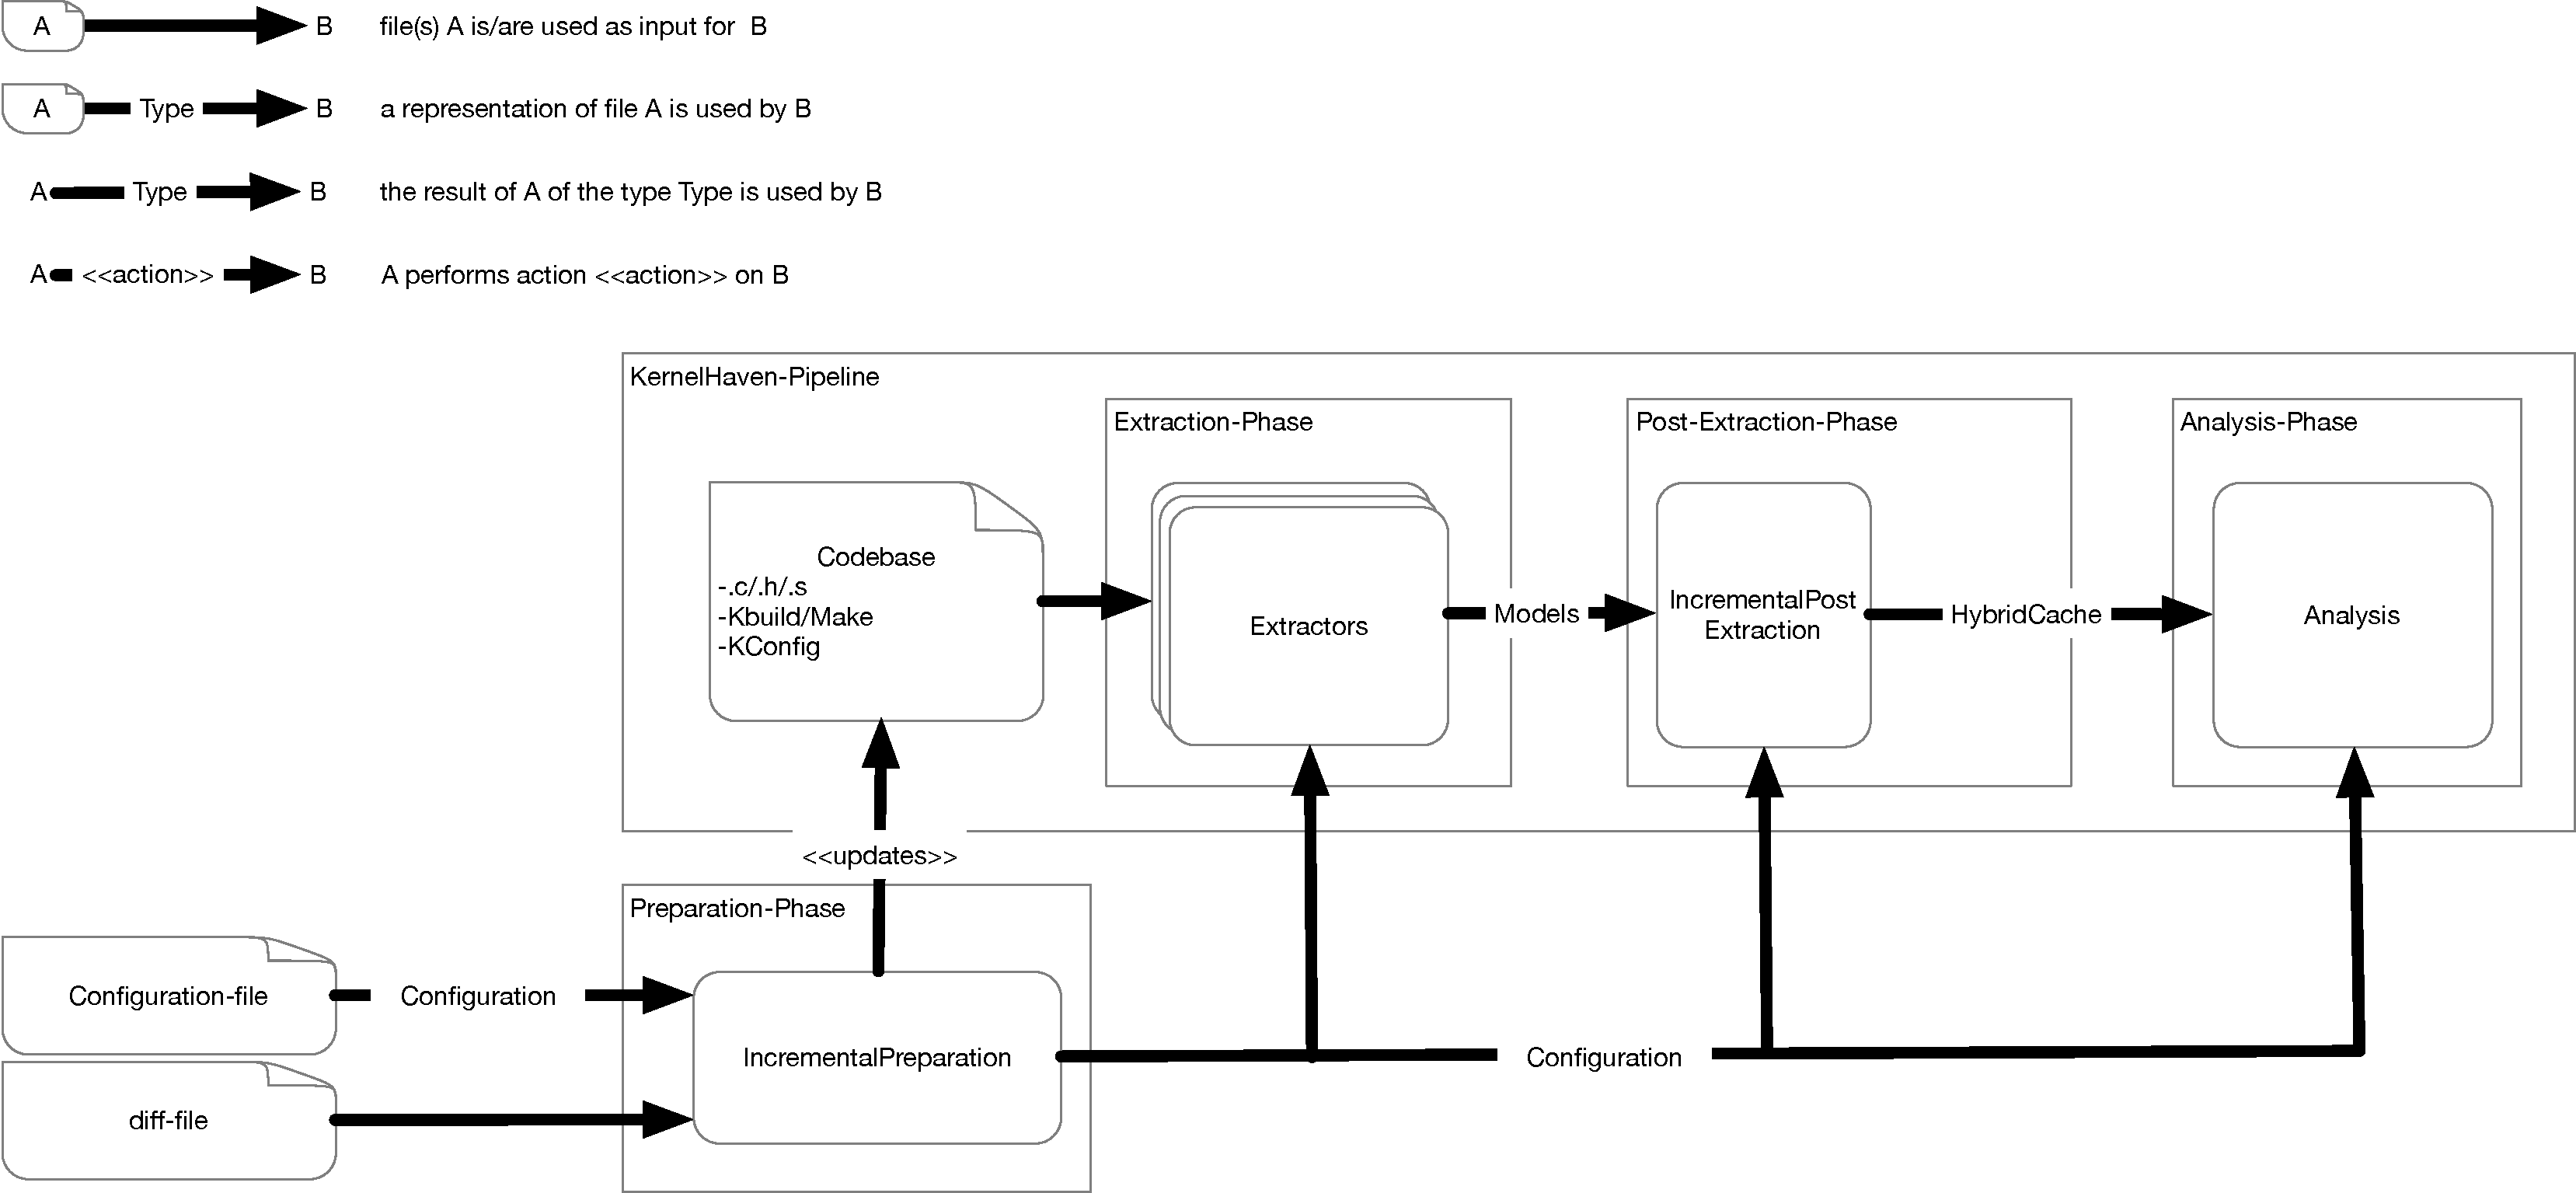
\includegraphics[width=1\textwidth]{img/KernelHavenIncremental.pdf}
  \end{minipage}
\end{figure}


\subsection{Implementation of the Preparation-Phase}\label{preparation-phase}

Because the definition of inputs for the extractors of the Preparation-Component needs to happen before the extraction and analysis itself, it makes sense to run them before an analysis is instantiated. With the \texttt{IPreparation}-interface, KernelHaven offers a mechanism to execute code before the rest of the infrastructure is started. Therefore it allows to modify the configuration that is initially described by a configuration-file. Furthermore other tasks independent of the modifications to the configuration such as applying changes to the codebase may also be executed.

An alternative to this approach would have been to configure extractors from within an analysis-plugin through the implementation of an \texttt{AnalysisComponent} or \texttt{IAnalysis}. In this case the analysis-plugin would have to care about the configuration of extractors and the content of the codebase on the filesystem. This is possible because KernelHaven is implemented as a pull-pipeline. The component at the very end of the pipeline could technically modify the way that prior components work. It would however represent a breach in the data-flow to have the last component modify the inputs and configuration for prior  components. 

In a non-incremental analysis, the definition of the configuration happens before the pipeline is started when writing the configuration-file. Some parameters of the configuration might get overwritten by command line parameters when the pipeline is set up by the \texttt{PipelineConfigurator}, the class responsible for putting all parts together before starting the pipeline - however the configuration is not directly modified from extractors or analyses. Using the \texttt{IPreparation}-interface preserves the data-flow within KernelHaven.

Furthermore, the the \texttt{IPreparation}-interface offers more flexibility to adjust the configuration of KernelHaven as all parts of the infrastructure - even the actual analysis-class itself - can be configured from within an \texttt{IPreparation}-implementation. Therfore the modifiability of the incremental infrastructure is higher than with analysis-classes which may only change the configuration for extractors.

For the incremental infrastructure, the \texttt{IncrementalPreparation}-class implements the \texttt{IPreparation}-interface and merges the changes described by the diff-file with the exisiting codebase. It then continues to  modify the configuration by defining the actual input-files upon which the extractors are run.


\subsubsection{Updating the Codebase}\label{git-apply}

The changes to the codebase are described through a git-diff file. While it is technically possible to create own implementations that apply those changes to files on the filesystem, we use the \texttt{git apply} command. \texttt{git apply} allows to apply changes in git-diff file to a given directory even if that directory is not a git repository. All that is required is command line call from within the folder on which the command should be applied:

\begin{lstlisting}[language=bash]
  $ git apply path/to/git.diff
\end{lstlisting}

 Furthermore \texttt{git apply} also allows to revert changes thereby ensuring the fulfillment of REQ \ref{req:rollback}:
 \begin{lstlisting}[language=bash]
  $ git apply --reverse path/to/git.diff
\end{lstlisting}
 
 A downside to using \texttt{git apply} is that it requires git to be installed on the system that KernelHaven is executed on. However because we assume a git-diff file as input (see REQ \ref{req:git-diff}), it is reasonable to assume that git is most likely already installed on the executing system.

Furthermore there are several advantages to using \texttt{git apply}. As the input is defined by the creation of a git-diff file through the \texttt{git diff} command, also using git to apply the changes ensures compatibility with the file. Therefore we assume that the existing git implementation is less prone to errors than an own implementation or other third party implementations. The integration of \texttt{git apply} results in a low implementation effort as command line calls can easily be realized through javas \texttt{ProcessBuilder}\footnote{ProcessBuilder documentation: \url{https://docs.oracle.com/javase/7/docs/api/java/lang/ProcessBuilder.html}}.

\subsubsection{Filtering of Input Files}\label{filtering-input}

After the codebase was updated, all files represeting variability within the revision that is to be analyzed are available for subsequent processing. To fulfill REQ \ref{req:early-filtering}, a filtering mechanism is implemented. Separate filters can be configured for code-, build-, and variability-files through te configuration-file.

One important resource that the filters use is an abstraction of the git-diff file that was used as input. This abstraction is implemented through the \texttt{DiffFile}-class.
An instance of the \texttt{DiffFile}-object contains an entry for each file that was affected by the changes described in the git-diff file that was used as input. For each entry, one of the following types of change is included:

\begin{itemize}
	\item \texttt{MODIFICATION} \\
	      indicates a modification of the file
	\item \texttt{ADDITION} \\
	      indicates the addition of the file
	\item \texttt{DELETION} \\
	      indicates the deletion of the file 
	\item \texttt{UNDEFINED} \\
	      the type of change should never be undefined. If it is, this indicates that the git-diff file was not properly translated into a \texttt{DiffFile}-object.
\end{itemize}

Furthermore the entries contain information on whether the variability is changed through the according git-diff file. So each entry is assigned one of the following markers aswell:

\begin{itemize}
	\item \texttt{CHANGE} \\
	      indicates changed variability
	\item \texttt{NO\_CHANGE} \\
	      indicates unchanged variability
	\item \texttt{NOT\_A\_VARIABILITY\_FILE}\\
	      indicates that the file was not considered to be a filetype that carries variability information
	\item \texttt{NOT\_ANALYZED}\\
	      indicates that the file was not analyzed at all for variability changes
\end{itemize}

Creating an abstraction of the git-diff file requires that the file itself is read and interpreted. This is done by a \texttt{DiffAnalyzer}, a class that takes the git-diff file used as input and translates it into a \texttt{DiffFile}-object. There are two existing DiffAnalyzers implemented within the incremental infrastructure: the \texttt{SimpleDiffAnalyzer} which only looks for the type of change without considering variability and the \texttt{VariabilityDiffAnalyzer} which also analyses for variability changes. The advantage of the \texttt{SimpleDiffAnalyzer} is that it is faster than the \texttt{VariabilityDiffAnalyzer}. \todo{give numbers here - how much slower? test on initial commit}
Therefore it makes sense to always use the \texttt{SimpleDiffAnalyzer} when variability-information is not needed for filtering.

The implementation of the \texttt{VariabilityDiffAnalyzer} relies on previous work which performed a commit based analysis of software product line evolution \cite{ComAn}. The tool used and implemented for this analysis  is called ComAn \cite{ComAn-tool}. Because the paper covers commits to the Linux kernel, the tool can process variability changes within the variablity files of the Linux kernel. 

ComAn is able to extract the number of lines for each changed file that is described in the git-diff file. This information is used within the \texttt{VariabilityDiffAnalyzer} to determine which files contain variability changes. 

The result of the \texttt{DiffAnalyzer} then gets passed to the filters together with the path to the codebase on the filesystem and a regular expression describing which files to include. The result is a list of all the paths that should be included for extraction. Because a separate filter is responsible for each type of model, three lists are created separately the extractors for build-, variability- and codemodel.
However currently only extractors for the codemodel can handle running on a subset of files within the codebase. As a result, both build- and variabilitymodel need to be extracted from scratch based on the entire codebase as soon as at least one file is included in the list.

Each of the three separate filters for the code-, build- and variabilitymodel can be configured individually but in some cases one implementation can also be reused for all models. This is because the regular expression may allow sufficient adjustments for each model type depending on the filter implementation. Any filter implementations must extend the abstract \texttt{InputFilter}-class. The following filters are included in the incremental infrastructure:

\begin{itemize}
\item \texttt{DefaultFilter} \\
    This filter lists all files within the directory of the codebase and filters them using the regular expression on the file-path. If all files representing  the build-, code- or variabilitmodel within the codebase are matched by the regular expression, this filter represents the off option described in REQ \ref{req:optimization}. 
\item \texttt{ChangedOnlyFilter} \\
    filters according to the change only option described in REQ \ref{req:optimization}. This filter takes the entries from the \texttt{DiffFile}-object where the file was either marked as Addition or Modification and then filters the file-paths for the regular expression.
\item \texttt{VariabilityChangesFilter} \\
    filters according to the variabilty change only option described in REQ \ref{req:optimization}. This filter filters similar to the \texttt{ChangedOnlyFilter} but only includes the files where the variability was marked as \texttt{CHANGE}.
\end{itemize}







%\Bibliography
\newpage

\bibliography{sources}


\end{document} 